% !TEX root = master.tex
\chapter{Evaluation der Ergebnisse}
\label{chapter:4}
\section{Ergebnisse}
\begin{table}[h]
	\centering
	\begin{tabularx}{\textwidth}{|c|X|c|}
		\hline
		\multirow{34}{*}[4ex]{\rotatebox[origin=c]{90}{\centering \textbf{Visualisierung}}} & \textbf{Anforderungen} & \textbf{Erfüllt} \\
		\cline{2-3}
		& Das Video wurde durch Python und Manim animiert und gerendert & $\square$ \\[4ex]
		& Die Länge des Videos überschreitet nicht 15 Minuten & $\square$ \\[4ex]
		& Das Video ist vollständig vertont & $\square$ \\[4ex]
		\cline{2-3}
		\multirow{44}{*}[10ex]{\rotatebox[origin=c]{90}{\centering \textbf{Implementierung}}} & Das Konzept von NEAT soll vollständig und verständlich sein & $\square$ \\[4ex]
		& Visualisierungsgrundlagen sollen berücksichtigt werden & $\square$ \\[4ex]
		& Ein roter Faden sollte erkennbar sein & $\square$ \\[4ex]
		& Das Video soll ansprechend animiert sein & $\square$ \\[4ex]
		\hline
		& NEAT Algorithmus implementieren und testen & $\square$ \\[4ex]
		& Lander durch NEAT Algorithmus steuern & $\square$ \\[4ex]
		& Aktionen aus 8-dimensionalen Input Vektoren ableiten & $\square$ \\[4ex]
		& Agent soll mindestens 200  Punkte erreichen & $\square$ \\[4ex]
		\cline{2-3}
		& Programm soll einfach und replizierbar sein & $\square$ \\[4ex]
		\hline
	\end{tabularx}
	\caption{Checkliste für funktionale und nicht funktionale Anforderungen}
\end{table}

Um das Projekt sachgemäß zu evaluieren wird im folgenden die Liste der Anforderungen, auf ihre Erfüllung, geprüft. 

Die Evaluierung der Visualisierung basiert auf dem eingereichten Video. (TODO LINK?) Anhand dessen kann gesehen werden, dass das gesamte Video im Manim Style erstellt wurde. Der zugehörige Quellcode ist in einem Github Repository dokumentiert. (TODO LINK?) Die Länge des Videos unterschreitet dabei 15 Minuten. Darüber hinaus ist das Video vollständig vertont. Basierend auf dem Feedback von Komilitonen ist das Konzept von NEAT verständlich rübergekommen, während der Ersteller des Videos aktiv darauf geachtet hat Visualisierungsgrundlagen wie Farbkomposition und Leserlichkeit eingehalten werden. Der rote Faden wird durch das zuvor angefertigte Story Board gewährleistet. Das Video wurde als angenehm zu schauen beurteilt, was zu großen Teilen auf dessen Animationen beruht. 

\begin{figure}[h] % 'h' bedeutet, dass LaTeX versuchen wird, das Bild an dieser Stelle einzufügen
	\centering % Zentriert das Bild horizontal
	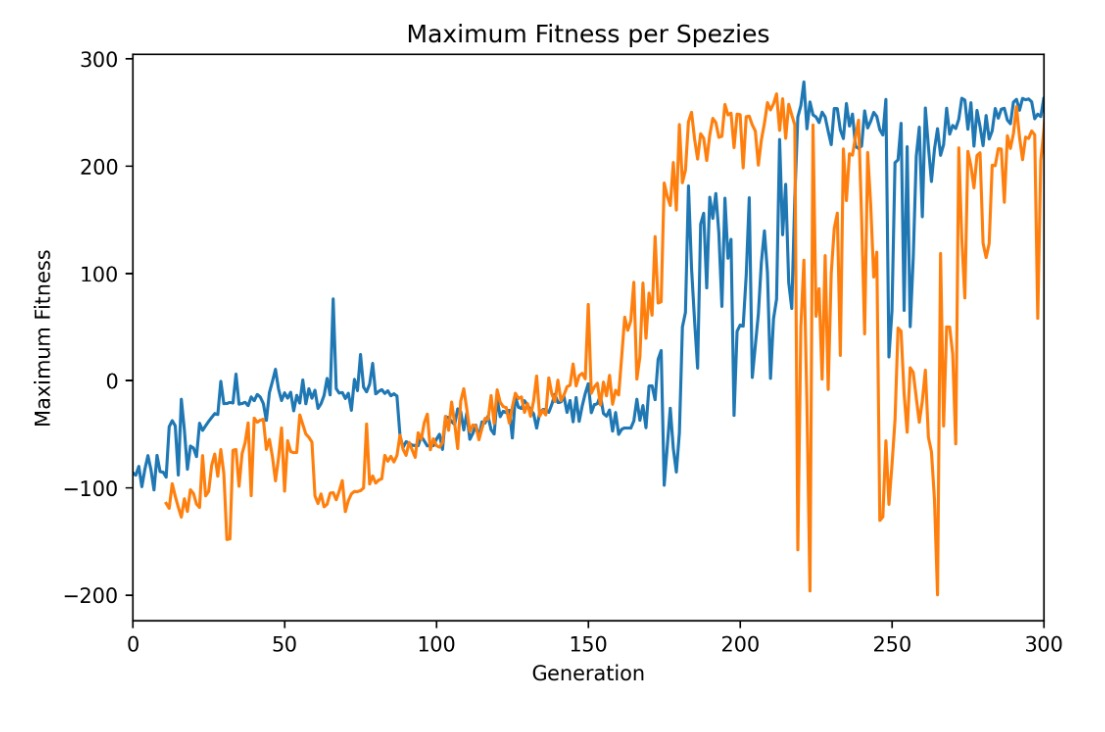
\includegraphics[width=1\textwidth]{\imagedir/species.jpg} % Ersetzen Sie 'meinbild.png' durch den Dateinamen Ihres Bildes
	\caption{Abbildung des Fitnessverlaufs der beiden besten Spezien} % Fügen Sie Ihre Bildbeschriftung hier ein
\end{figure}

---- Genauigkeit des Landers
---- Vergleich zu anderen Methoden/Baseline
---- Entstandenes Video mit Bezug auf psychologische Effekt von zuvor (Baseline)

\section{Handlungsempfehlungen}
(1 Seite)
---- NEAT klappt wunderbar damit
---- Limitationen sind ...
---- Das Feld hat Zukunft weil ...